% The draft script for IEEE Transactions on Affective Computing
% Version: 1.0
% Due date (Abstract): N.A.
% Due date (Full Paper): N.A.
\documentclass[10pt,journal,compsoc]{IEEEtran}


% ========================= PACKAGES ============================
% CITATION PACKAGES
% IEEE Computer Society needs nocompress option
\ifCLASSOPTIONcompsoc
  \usepackage[nocompress]{cite}  % Computer Society
\else
  \usepackage{cite}              % Normal
\fi

% GRAPHICS RELATED PACKAGES
\ifCLASSINFOpdf
  \usepackage[pdftex]{graphicx}
  \graphicspath{{assets/}{profiles/}}          % set paths
  \DeclareGraphicsExtensions{.pdf,.jpeg,.png}  % set extensions
\else
  \usepackage[dvips]{graphicx}
  \graphicspath{{assets/}{profiles/}}
  \DeclareGraphicsExtensions{.eps}
\fi

% MATH PACKAGES
\usepackage{amsmath}
% Note that the amsmath package sets \interdisplaylinepenalty to
% 10000 thus preventing page breaks from occurring within
% multiline equations. Use following command after loading
% amsmath to restore such page breaks as IEEEtran.cls normally
% does.
% \interdisplaylinepenalty=2500

% ALGORITHM
% \usepackage{algorithmic}
% algorithmic.sty provides an algorithmic environment. You can
% use in-text or within a figure environment to provide for a
% floating algorithm.
% Do NOT use algorithm.sty or algorithm2e.sty.

% ALIGNMENT PACKAGES
\usepackage{array}
% array.sty patches and improves the standard LaTeX2e array and
% tabular environments. All users are strongly advised to use an
% enhanced set of table tools.

% SUBFIGURE PACKAGES
\ifCLASSOPTIONcompsoc
  \usepackage[caption=false,font=footnotesize,labelfont=sf,textfont=sf]{subfig}
\else
  \usepackage[caption=false,font=footnotesize]{subfig}
\fi
% subfig.sty is the modern replacement for subfigure.sty.
% However, subfig.sty requires and automatically loads aption.sty
% which will override IEEEtran.cls handling of captions and this
% will result in non-IEEE style figure/table captions.
% To prevent this problem, be sure and invoke subfig.sty's
% "caption=false" package option.
% Note that the Computer Society format requires a sans serif
% font and thus the need to invoke different subfig.sty package
% options depending on whether compsoc mode has been enabled.
% \begin{figure}[!t]
%   \centering
%   \subfloat[Subfig I]{\includegraphics[width=2.5in]{subfig_1}%
%   \label{subfig_1}}
%   \hfil
%   \subfloat[Subfig II]{\includegraphics[width=2.5in]{subfig_2}%
%   \label{subfig_2}}
%   \caption{Simulation results for the network.}
%   \label{subfig}
% \end{figure}

% FLOAT PACKAGES
% \usepackage{stfloats}
% stfloats.sty gives LaTeX2e the ability to do double column
% floats at the bottom of the page as well as the top. (e.g.,
% "\begin{figure*}[!b]" is not normally possible in LaTeX2e).
% It also provides a command \fnbelowfloat to enable the
% placement of footnotes below bottom floats (the standard
% LaTeX2e kernel puts them above bottom floats). This is an
% invasive package which rewrites many portions of the LaTeX2e
% float routines. It may not work with other packages that modify
% the LaTeX2e float routines.
% Do not use the stfloats baselinefloat ability as the IEEE does
% not allow \baselineskip to stretch. Authors submitting work to
% the IEEE should note that the IEEE rarely uses double column
% equations and that authors should try to avoid such use. Do not
% be tempted to use the cuted.sty or midfloat.sty packages as the
% IEEE does not format its papers in such ways. Do not attempt to
% use stfloats with fixltx2e as they are incompatible. Instead,
% use Morten Hogholm'a dblfloatfix which combines the features of
% both fixltx2e and stfloats:
% \usepackage{dblfloatfix}

% URL & HYPERLINK PACKAGES
\usepackage{url}
% url.sty provides better support for handling and breaking URLs.
% Basically, \url{my_url_here}.

% MY PACKAGES
\usepackage{amssymb}
\usepackage{booktabs}
\usepackage{xspace}
\makeatletter
\DeclareRobustCommand\onedot{\futurelet\@let@token\@onedot}
\def\@onedot{\ifx\@let@token.\else.\null\fi\xspace}
\def\eg{\emph{e.g}\onedot} \def\Eg{\emph{E.g}\onedot}
\def\ie{\emph{i.e}\onedot} \def\Ie{\emph{I.e}\onedot}
\def\cf{\emph{c.f}\onedot} \def\Cf{\emph{C.f}\onedot}
\def\etc{\emph{etc}\onedot} \def\vs{\emph{vs}\onedot}
\def\wrt{w.r.t\onedot} \def\dof{d.o.f\onedot}
\def\etal{\emph{et al}\onedot}
\makeatother
\usepackage{xcolor}
\usepackage{multirow}
\usepackage{threeparttable}

% correct bad hyphenation here
\hyphenation{net-works multi-party}


% ====================== TITLE & AUTHORS ========================
\begin{document}
\title{Engagement Estimation of the Elderly\\
from Wild Multiparty Human-Robot Interaction}

% Author(s)
% `~` keeps an author's name from being broken across two lines.
% Use `\thanks` to access the footnote. A separate `\thanks`
% must be used for each paragraph.
% `\IEEEcompsocitemizethanks` is a special `\thanks` that
% produces the bulleted lists the Computer Society journals use
% for "first footnote" author affiliations.
% Use `\IEEEcompsocthanksitem` which works much like `\item` for
% each affiliation group.
% Use `~\IEEEmembership{}` just following the author name for
% declaring the membership: `~\IEEEmembership{Fellow,~IEEE}`.
\author{
  Zhijie~Zhang,
  Jianmin~Zheng,
  and~Nadia~Magnenat~Thalmann% <- this % stops a space

  \IEEEcompsocitemizethanks{
    \IEEEcompsocthanksitem Z. Zhang and J. Zheng are with the School of Computer Science and Engineering, Nanyang Technological University, Singapore.\protect\\
    % use \protect\\ to get a newline within \thanks.
    E-mail: {\{zhijie002, asjmzheng\}@e.ntu.edu.sg}
    \IEEEcompsocthanksitem N. M. Thalmann is with the MIRALab, University of Geneva, Switzerland.\protect\\
    E-mail: {thalmann@miralab.ch}
    \IEEEcompsocthanksitem N. M. Thalmann is with the MIRALab, University of Geneva, Switzerland.\protect\\
    E-mail: {thalmann@miralab.ch}
    \IEEEcompsocthanksitem N. M. Thalmann is with the MIRALab, University of Geneva, Switzerland.\protect\\
    E-mail: {thalmann@miralab.ch}
  }% <-this % stops an unwanted space

  \thanks{Manuscript received April 19, 2005; revised August 26, 2015.}
}

% Paper Headers
\markboth{Journal of \LaTeX\ Class Files,~Vol.~14, No.~8, August~2015}%
{Shell \MakeLowercase{\etal}: Bare Demo of IEEEtran.cls for Computer Society Journals}
% The only time the second header will appear is for the odd
% numbered pages after the title page when using the twoside
% option.
% Note that you probably will NOT want to include the author's
% name in the headers of peer review papers. You can use
% \ifCLASSOPTIONpeerreview for conditional compilation here if
% you desire.

% The publisher's ID mark at the bottom of the page is less
% important with Computer Society journal papers as those
% publications place the marks outside of the main text columns
% and, therefore, unlike regular IEEE journals, the available
% text space is not reduced by their presence. If you want to
% put a publisher's ID mark on the page you can do it like this:
% \IEEEpubid{0000--0000/00\$00.00~\copyright~2015 IEEE}
% or like this to get the Computer Society new two part style.
% \IEEEpubid{\makebox[\columnwidth]{\hfill 0000--0000/00/\$00.00~\copyright~2015 IEEE}%
% \hspace{\columnsep}\makebox[\columnwidth]{Published by the IEEE Computer Society\hfill}}
% Remember, if you use this you must call \IEEEpubidadjcol in
% the second column for its text to clear the IEEEpubid mark
% (Computer Society jorunal papers don't need this extra
% clearance.)

% Use for special paper notices
%\IEEEspecialpapernotice{(Invited Paper)}


% ==================== ABSTRACT & KEYWORDS ======================
% 1. Background
% 2. Problem, motivation, and challenges
% 3. Approach
% 4. Results
\IEEEtitleabstractindextext{
\begin{abstract}
With the improvement of the standard of living, humans have the increasing longevity, but improving the quality of life for the elderly remains a challenge. In recent years, many researchers have studied the use of assistive agents in clinical treatment and nursing homes, where the concept of engagement has been proposed and has become an essential indicator. However, traditional engagement estimation often requires expert involvement and is in controlled dyadic interaction environment. In this paper, we use real-world video recordings to estimate old people's engagement in a multiparty human-robot interaction scenario. For this purpose, we place a humanoid robot in a non-profit nursing home, where the elderly are accompanied by nurses and engage in spontaneous conversations with the robot. We propose a framework based on self-attention mechanism and graph attention neural networks, which uses videos as input to automatically generate an engagement value between 0 and 1. The model is built on the components of engagement discussed in geriatric psychiatry (behavioral, affective, and visual) and video representations for interaction understanding (group and individual levels). We test the proposed framework using 22 wild multiparty elderly-robot interaction videos by answering the following questions: What is the engagement value of the elderly? Who makes up the main interaction group? Could the information from other participants help make an estimation? The results show that our model is capable of detecting the key participants and estimating the engagement of the elderly. Moreover, information from the surroundings can considerably improve the estimation results. % The code is available at \url{}.
\end{abstract}

\begin{IEEEkeywords}
Human-Robot Interaction, Engagement Estimation, Affective Computing, Multiparty Interaction, the Elderly.
\end{IEEEkeywords}
}


% ======================== MAKE TITLE ===========================
\maketitle
% To allow for easy dual compilation without having to reenter
% the abstract/keywords data, the \IEEEtitleabstractindextext
% will not be used in maketitle, but will appear (i.e., to be
% "transported") here as \IEEEdisplaynontitleabstractindextext
% when the compsoc/transmag modes are not selected OR conference
% mode is selected. \IEEEdisplaynontitleabstractindextext has no
% effect when using compsoc/transmag under a non-conference mode.
\IEEEdisplaynontitleabstractindextext

% For peer review, you can put extra information on the cover
% page as needed.
% \ifCLASSOPTIONpeerreview
% \begin{center} \bfseries EDICS Category: 3-BBND \end{center}
% \fi
%
% For peer review, this command inserts a page break and
% creates the second title. It will be ignored for other modes.
\IEEEpeerreviewmaketitle


% ======================= INTRODUCTION ==========================
% 1. Background & Motivation
% 2. Problem Statement
% 3. Challenges & Existing works
% 4. Our Approach & Contributions

% Computer Society journal (but not conference) papers place the
% first section heading ABOVE the main text. You can achieve this
% with the provided \IEEEraisesectionheading{} command.

% The very first letter is a 2 line initial drop letter followed
% by the rest of the first word in caps (small caps for compsoc).
% Single letter:
% \IEEEPARstart{A}{demo} file is ...
% Two and more letters:
% \IEEEPARstart{T}{his} demo file is ...
% \IEEEPARstart{T}{}his demo file is ...

\IEEEraisesectionheading{
\section{Introduction}
\label{s:Introduction}
}

\IEEEPARstart{T}{he} degree and pace of population ageing have increased dramatically in the past decades. According to the World Health Organization, the proportion of the world's population over 60 years will nearly double from 12\% in 2015 to 22\% in 2050~\cite{WHO2021Ageing}. In addition, old people usually experience significant declines in physical and cognitive capacities, so round-the-clock medical and psychological care are important for them. Many studies claimed that deploying robots in the healthcare setting is a possible solution, \eg, they support people with dementia (PwD) and their caregivers by reducing costs and improving the independence of the old people~\cite{Ghafurian2021Social, Perugia2020ENGAGEDEM}.

This work centers on the elderly-robot interaction and attempts to come up with an approach to estimating the engagement of the elderly. Here, engagement is defined as the inner state of a participant attributing to being together with the other participants and continuing the interaction~\cite{Poggi2013Mind}. Many studies have approved the importance of engagement in both human-human interaction (HHI) and human-robot interaction (HRI)~\cite{Jones2018Engagement}. By giving robots the ability to recognize engagement state, they are able to generate socially acceptable behavior, form long-term connections, and more importantly to design activities for seniors that allow them to use their skills and feel a sense of belonging.

Automated engagement estimation is comparable to affective computing and behavior recognition in computer vision area, but it goes a step further to probe the inner intention behind the apparent behavior and emotion. Previous works have been proposed to estimate engagement in various scenarios such as general HRI~\cite{Salam2017Fully, Celiktutan2019Multimodal, BenYoussef2019Early, Saleh2021Improving}, museum tour guide~\cite{DelDuchetto2020Are}, and classroom or distance learning~\cite{BenEliyahu2018Investigating, Zhu2020Multirate, Rudovic2019Personalized, Sumer2021Multimodal, Monkaresi2017Automated, Abedi2021Affectdriven, Gao2020NGage}, toddlers and seniors healthcare~\cite{Anagnostopoulou2021Engagement, Jain2020Modeling, Jones2018Engagement, Steinert2020Engagement}. Conventional approaches use nonverbal cues such as proxemics, body pose, gaze patterns, facial expressions, and context information to build engagement estimation classifiers. However, as shown in Fig.~\ref{f:interaction_sample}, when the research is expanded to some special populations or more complex circumstances, such challenging work is still lacking. This work attempts to confront these challenging issues:
\begin{enumerate}
  \item[Q1] Given that the non-verbal signals from \textbf{the elderly}, which alter in facial shape and patterns of body behaviors along with aging~\cite{Guo2013Facial, Folster2014Facial}, can we use a pure computer vision approach to accurately estimate engagement state?
  \item[Q2] From dyadic to \textbf{multiparty HRI}, how to understand the dynamics and stability of the interaction in such a scenario? Can we propose an automated approach to analyze an old person?
  \item[Q3] In unconstrained \textbf{wild} space, how to understand the complex environment (moving people, bad lighting, and confusing objects)?
\end{enumerate}

To this end, we propose a novel deep learning framework for automatically estimating engagement from videos of real-world multiparty elderly-robot interactions. Specifically, as shown in Fig.~\ref{f:architecture}, our approach takes video sequences as input and output the estimated engagement state. \textcolor{blue}{For each image, we first perform human detection and pose estimation, on the basis of which we implement 3D pose reconstruction. Through the reconstructed scenes and the positions of people in different frames, we explore the relationships between people, and then obtain the main groups interacting with the robot, after which we continue the scale down to the main elderly, which is done through facial recognition. We perform feature extraction and preliminary estimation at each of these three scales. Specifically, on the global scale, we use the ResNet-50~\cite{He2016Deep} as the backbone with self-attention mechanism~\cite{Wang2018NonLocal}. For the group branch, we utilize both image features from pre-trained convolutional networks (CNNs) and high-level social features such as body pose, facial landmarks as the node information of graph attention networks (GATs)~\cite{Velivckovic2017Graph} where the edges model the interactions among individuals. Individual estimation is similar to group branch but without GATs. The final estimation is a combination of these estimations.} The main contributions of the paper are

\begin{itemize}
\item We propose an automated approach that analyzes wild multiparty HRI videos and estimates the engagement of the elderly.
\item We explore three scales' information and approve that the combination of global, group, and individual information achieves better performance than only using individual features.
\end{itemize}

This paper is organized as follows. Sec.~\ref{s:Related_Work} presents the related work of engagement estimation in HRI, especially for the elderly. Sec.~\ref{s:Engagement_Estimation_of_the_Elderly} describes our proposed approach for estimating the engagement in a real-world scenario and the method of detecting main conversation group members. In Sec.~\ref{s:Datasets}, we elaborate the dataset we collected and used for our experiments, as well as the annotation process. The details of the implementation, evaluation metrics, and main results are presented and discussed in Sec.~\ref{s:Experiments}. 
Finally, Sec.~\ref{s:Conclusions} summarizes the paper and outlines possible future work.

\begin{figure}[t]
  \centering
  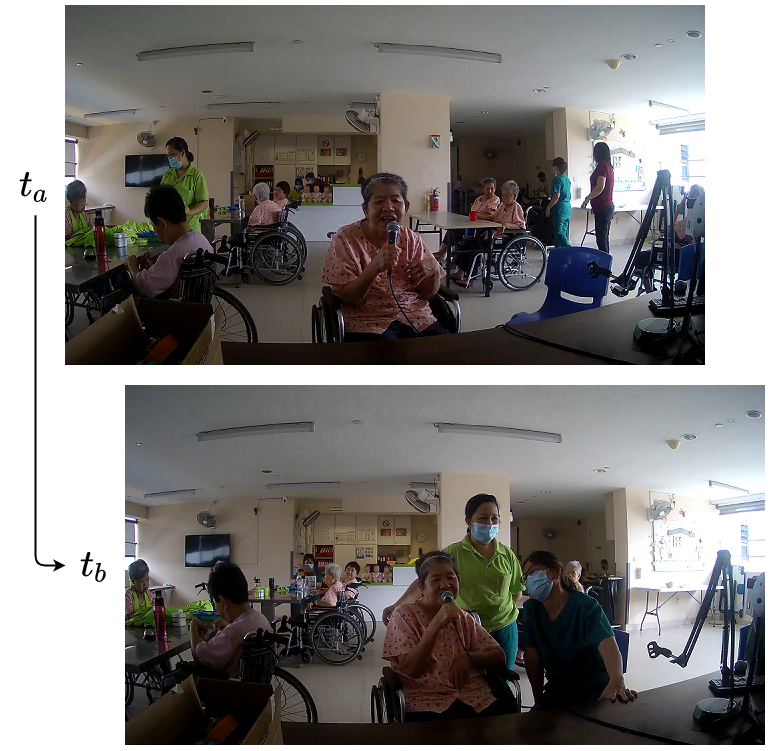
\includegraphics[width=\linewidth]{assets/interaction_sample.drawio.png}
  \caption{Two sample frames from a video recording of real-world multiparty HRI, demonstrating conversation dynamics (from one to three participants) and unconstrained environment (open space and free-moving background people). The video is recorded from robot ego-view, $t_a$ and $t_b$ denoting two time stamps.}
  \label{f:interaction_sample}
\end{figure}


% ======================= RELATED WORK ==========================
\section{Related Work}
\label{s:Related_Work}

The estimation of engagement encompasses a wild range of fields from computer vision to psychological science and psychiatric nursing. The related work provided in this section includes the concepts of engagement (Sec.~\ref{subs:What_Is_Engagement}) and the methodology for automatically estimating engagement (Sec.~\ref{subs:Automated_Engagement_Estimation}).

\begin{table*}[t]
  \renewcommand{\arraystretch}{1.3}
  \centering
  \caption{Comparison of Engagement Estimation Approaches}
  \label{t:references}
  \begin{threeparttable}[b]
  \begin{tabular}{p{0.04\linewidth}p{0.08\linewidth}p{0.18\linewidth}p{0.15\linewidth}p{0.18\linewidth}p{0.22\linewidth}}
  \toprule
  \textbf{Paper} &
  \textbf{Scenario} &
  \textbf{Participant(s)}\tnote{1} &
  \textbf{Input Modality(s)}\tnote{2} &
  \textbf{Approach} \tnote{3} &
  \textbf{Output}\tnote{4} \\
  \midrule
  \cite{Salam2017Fully} &
  HRI &
  multiparty &
  vis, dpt, per &
  SVM \& RF &
  $\hat{y} \in$ \{Eng, NEng\} \\
  \cite{BenYoussef2019Early} &
  HRI &
  individual/group &
  vis, aud &
  LR &
  $\hat{y} \in$ \{NBrk, Brk\} \\
  \cite{Monkaresi2017Automated} &
  HCI &
  individual, age (20-60) &
  vis &
  NB &
  $\hat{y} \in$ \{Eng, NEng\} \\
  \cite{Gao2020NGage} &
  HHI &
  group, age (15-17) &
  phy, env &
  LightGBM &
  $\hat{y} \in$ [1, 5] \\
  \midrule
  \cite{Saleh2021Improving} &
  HRI &
  individual/group &
  vis &
  I3D &
  $\hat{y} \in$ \{Eng, NEng\} \\
  \cite{DelDuchetto2020Are} &
  HRI &
  individual/group &
  vis &
  CNNs + LSTM &
  $\hat{y} \in$ [0, 1] \\
  \cite{Zhu2020Multirate} &
  HCI &
  individual, age (19-27) &
  vis &
  GRU &
  $\hat{y} \in$ \{HEng, Eng, BEng, NEng\} \\
  \cite{Rudovic2019Personalized} &
  HRI &
  individual, age (4-6) &
  vis &
  RL &
  $\hat{y} \in$ \{HEng, MEng, LEng\} \\
  \cite{Sumer2021Multimodal} &
  HHI &
  group, students &
  vis &
  MLP \& LSTM &
  $\hat{y} \in$ \{HEng, MEng, LEng\} \\
  \cite{Anagnostopoulou2021Engagement} &
  HRI &
  individual/group, child &
  vis, dpt &
  CNNs \& LSTM &
  $\hat{y} \in$ \{Eng, MEng, NEng\} \\
  \cite{Steinert2020Engagement} &
  HCI &
  individual, PwD &
  vis &
  LSTM &
  $\hat{y} \in$ \{Eng, MEng, NEng\} \\
  \cite{Guhan2020ABCNet} &
  HHI/HCI &
  individual &
  vis, aud, txt &
  GANs &
  $\hat{y} \in$ \{Eng, NEng\} \\
  \midrule
  \textbf{Ours} &
  HRI &
  multiparty, PwD &
  vis &
  I3D + Attention + GATs &
  $\hat{y} \in$ [0, 1] \\
  \bottomrule
  \end{tabular}
  \begin{tablenotes}
    \item [1] The difference between multiparty and group is that multiparty treats participants separately but group is a whole.
    \item [2] Modalities: vis = visual, dpt = depth, per = personality, aud = audio, phy = physiological, env = environmental, and txt = text.
    \item [3] The symbol \& indicates using both and comparing with each other. + means combining to form a framework.
    \item [4] $\hat{y}$ represents the inferred engagement label or value. For classification, Eng = Engage, Brk = Breakdown. The letters before Eng and Brk are N = Not, H = Highly, B = Barely, and M = Medium.
  \end{tablenotes}
 \end{threeparttable}
\end{table*}

\subsection{What Is Engagement?}
\label{subs:What_Is_Engagement}

\subsubsection{Definition of Engagement}

Before we discuss engagement in HRI, let's clarify the definition of engagement first. According to Oertel \etal~\cite{Oertel2020Engagement}, the notion of engagement is ambiguous among different research domains, which are regarded as a state or a process. Participants are either engaged or not engaged in terms of state, but, by contrast, a classical process definition was proposed by Sidner \etal~\cite{Sidner2005Explorations} as the process through which interactors establish, maintain, and complete their perceived connection to each other during an interaction.

It is important to note that the term \textbf{\textit{state}} is used here to distinguish it from \textit{process}, which represents objectively observed facts in HHI or HRI, \ie, the participants are within interaction or not. This is different from the \textbf{\textit{state}} used in the phrases\textemdash \textit{engagement state estimation} or \textit{inner state}\textemdash depicting participants' the whole mental, feeling, emotional, and cognitive states. In this paper, we adopt the definition of engagement from~\cite{Poggi2013Mind}, which is the participant's inner state of being together with other participants and continuing the interaction.

\subsubsection{Components of Engagement}

According to~\cite{Castellano2009Detecting, Guhan2020ABCNet, Sumer2021Multimodal, Christenson2012Handbook, OBrien2008What, CohenMansfield2011Comprehensive, Archambault2017Joint, BenEliyahu2018Investigating, Corrigan2016Engagement, Perugia2020ENGAGEDEM}, engagement contains different components. The distinctions and definitions of these components vary across research areas. In general, common components include: behavioral, affective, visual, verbal, social, and cognitive. Moreover, these components are not mutually exclusive but often overlap with each other.

\begin{itemize}
  \item \textbf{Behavioral:} involves observable behaviors such as approaching, touching, avoiding, or hitting, \etc
  \item \textbf{Affective:} is defined as the affective reactions that are usually represented by the valence and arousal.
  \item \textbf{Visual:} encompasses actions involving the eyes and head, such as maintaining contact or appearing inattention to others or materials.
  \item \textbf{Verbal:} reflects the sounds and semantic information towards other participants.
  \item \textbf{Cognitive:} pertains to the psychological investment and effort allocation of the person in order to fully comprehend the situation.
  \item \textbf{Social:} includes social activities such as encouraging or disrupting others.
\end{itemize}

In our work, since our target is to estimate the engagement of the elderly with a humanoid robot in casual conversation via a pure computer vision approach, we select behavioral, affective, and visual engagement. Because of the input modality, the verbal component is eliminated, while the cognitive and social components are overlooked due to the participant's physical and mental conditions.

\subsubsection{Engagement in Different Scenarios}

Engagement estimation is studied in many disciplines and interaction scenarios. A simple taxonomy is based on the type of interactors: engagement in HHI or HRI. Although participants perform and feel differently in HHI and HRI, the estimation of engagement in these two contexts is similar in methods. For example, in~\cite{Oertel2021EngagementAware}, Oertel \etal demonstrated the knowledge from the HHI can be applied to HRI. Therefore, we will discuss both in Sec.~\ref{subs:Automated_Engagement_Estimation}.

On the other hand, the application scenarios of engagement estimation are also different, such as everyday conversations, healthcare, and learning situations, among others. In different scenarios, engagement is often expressed differently, while the dominance of its components varies. As a result, the corresponding estimation methods are different and hard to make comparison, let alone find a universal approach.

\subsection{Automated Engagement Estimation}
\label{subs:Automated_Engagement_Estimation}

In terms of the methodology, traditional approaches~\cite{Salam2017Fully, Celiktutan2019Multimodal, BenYoussef2019Early, Monkaresi2017Automated, Gao2020NGage} extract high-level social features, \eg, body pose, facial expressions, gaze, and task-related information, followed by a machine learning classifier. Several papers are heuristic, demonstrating that specific features are meaningful by using and comparing unimodal and multimodal feature combinations. Recently, with the development of computer vision, more and more deep learning methods have been proposed~\cite{Saleh2021Improving, DelDuchetto2020Are, Zhu2020Multirate, Guhan2020ABCNet, Rudovic2019Personalized, Sumer2021Multimodal, Anagnostopoulou2021Engagement}. A summary of the literature is shown in Table~\ref{t:references}, grouped by estimation approaches.

\subsubsection{Machine Learning Classifiers}

In general HRI, Salam \etal~\cite{Salam2017Fully} classified engagement using support vector machines (SVM) and random forests (RF), depending on predicted personality in a triadic interaction. They advanced the concept of engagement to the group level and claimed that categorization of engagement based on individual and interpersonal features without personality is insufficient. A similar work is from Celiktutan \etal~\cite{Celiktutan2019Multimodal}. Ben-Youssef \etal~\cite{BenYoussef2019Early} investigated engagement in HRI from the breakdown perspective, \ie, users leave before the expected end. They extracted nonverbal multimodal data such as the distance to the robot, gaze and head motion, facial expressions, and audio. A logistic regression (LR) classifier is used. 

Another widely investigated situation is online and in-class learning. Monkaresi \etal~\cite{Monkaresi2017Automated} explored engagement where students complete an online writing activity. Heart rate, animation units (AUs), and local binary patterns are extracted and fed to a set of classifiers like Naive Bayes (NB). Gao \etal~\cite{Gao2020NGage} predicted high school students' learning engagement including emotional, behavioral, and cognitive engagement in real-world class. They used a set of features from wearable and indoor weather sensors to infer students' engagement.

\subsubsection{Deep Neural Networks}

The aforementioned approaches require expert design of input features and cannot deal with large feature dimensions efficiently, \eg, when pixel values from face images are used as input. Del Duchetto \etal~\cite{DelDuchetto2020Are} propose a regression model based on CNNs and Long Short-Term Memory (LSTM) networks, which allows robots to compute the engagement from ego-view HRI videos. The model is built on a long-term dataset from an autonomous tour guide robot in a museum. Zhu \etal~\cite{Zhu2020Multirate} presented an attention-based Gated Recurrent Unit (GRU) network to predict engagement of students learning online. Taking the advantage of the published dataset from ~\cite{BenYoussef2019Early}, Saleh \etal~\cite{Saleh2021Improving} applied Inflated 3D ConvNets (I3D) architecture to predict engagement state in an end-to-end way.

In addition, Anagnostopoulou \etal~\cite{Anagnostopoulou2021Engagement} estimated the engagement of children with autism spectrum disorder when they interact with robots. They compared architectures of AlexNet, CNNs, and LSTM using 2D or 3D poses. Rudovic \etal~\cite{Rudovic2019Personalized} proposed a personalized reinforcement learning (RL) approach to estimate engagement level (low, medium, high) from videos of child-robot interactions, where queried videos are labeled offline by experts, and used to personalize the policy and engagement classifier to a target child over time.

For HHI, Sumer \etal~\cite{Sumer2021Multimodal} utilized video recordings of offline classes to get attentional and emotional engagement features, and then applied SVM, RF, multilayer perceptron (MLP), and LSTM to predict students' engagement levels. Guhan \etal~\cite{Guhan2020ABCNet} described a multimodal GAN-based approach, called ABC-Net, to identify engagement from online dyadic HHI recordings. They utilized three-branch networks to gain valence and arousal first and then generate engagement labels.

\subsection{Engagement for the Elderly}

In geriatric psychiatry, research on engagement is well established. In~\cite{Cohen2009Engagement}, the authors described an Observational Method of Engagement (OME) for persons with dementia, which is one of the most well-known tools many studies used to measure engagement~\cite{Trahan2014Systematic}. Followed by this concept, Jones \etal~\cite{Jones2018Engagement} developed the Engagement of a Person with Dementia Scale (EPWDS) towards psychosocial activities by assessing the behavioral and emotional expressions and responses. In~\cite{Perugia2020ENGAGEDEM}, ENGAGE-DEM, an affective computing framework is presented, specifying the components of engagement in HRI.

Moreover, robotic and computer assistance has been approved as an effective intervention. Moyle \etal~\cite{Moyle2017Use} developed a robot seal for PwD. They found that participants were more engaged with it compared to a toy, and robot seal is more effective than usual care in improving mood states and agitation. Similarly, Feng \etal~\cite{Feng2021ContextEnhanced} introduced an interactive system involving a display and a robotic sheep to engage PwD. They claimed that multimodal stimuli play a significant role in promoting engagement.

However, all the previously mentioned engagement estimation methods require expert involvement. For automated estimation methods, Steinert \etal~\cite{Steinert2020Engagement} presented a vanilla LSTM model to predict emotional engagement based on visual (extracted OpenFace~\cite{Baltrusaitis2018OpenFace} and \and VGGFace~\cite{Parkhi2015Deep} facial features) and contextual information (daytime, wellbeing, \etc).


% ========================= APPROACH ============================
% 1. Overview
% 2. Feature extraction
% 3. Pipeline and network structure
% 4. Multiparty transition
\section{Engagement Estimation of the Elderly}
\label{s:Engagement_Estimation_of_the_Elderly}

\begin{figure}[t]
  \centering
  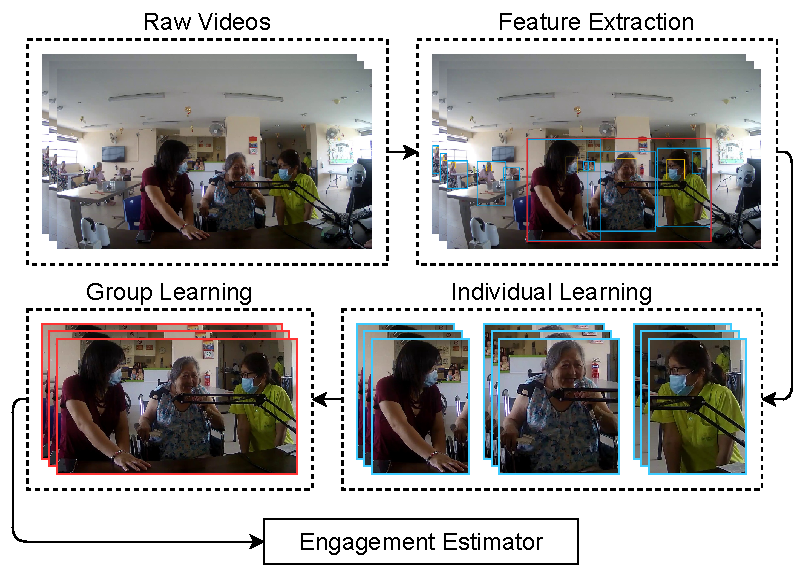
\includegraphics[width=\linewidth]{assets/architecture.drawio}
  \caption{Overview of the proposed engagement estimation architecture. This architecture is composed of four modules, (i) Feature Extraction, (ii) Individual Learning, (iii) Group Learning, and (iv) Engagement Estimator.}
  \label{f:architecture}
\end{figure}

In this section, we describe our proposed engagement estimation approach of the elderly from wild multiparty HRI. We use raw video recordings of the elderly-robot interaction, described in Sec.~\ref{s:Datasets}. Formally, we define the dataset as $\mathcal{V} = \{V_1, ..., V_m, ..., V_M\}$, where $V_m$ is video recordings of interaction session $i$. For every interaction session, normally there is only one old participant $p$. Moreover, each interaction session includes $K$ video clips, denoted as $V_m = \{v_m^1, ..., v_m^k, ..., v_m^K\}$, where $K$ may vary per session. Lastly, each video clip is associated with a target ground truth $y_m^k \in [0, 1]$, corresponding to the elderly's engagement state. From 0 to 1, the output value indicates an increase in engagement. Given these data, our goal is to output an estimated value of engagement $\hat{y}_m^k$ that is as close as possible to the ground truth.

As mentioned before, our task is very challenging and complicated, because we contend with the background clutter and accurately capture the inner engagement state of a specific old person from a dynamic multiparty interaction. To address them, we design a novel framework for engagement estimation of the elderly. The overview of the architecture is illustrated in Fig.~\ref{f:architecture}. First, we use the pre-trained I3D as the backbone to obtain spatio-temporal representations of the input videos. Then, we design an individual learning module for refining individual features by adding a self-attention mechanism. Following that, we construct GATs to learn the relationships within the main group and group-level information. Finally, we make inference through an estimator outputting a value that reflects the elderly's engagement state.

In comparison to other related studies, the main advantage of our approach is that we attempt to provide answers the three questions raised in Sec.~\ref{s:Introduction}. First, because the facial features and body movements of older adults are difficult to recognize, we design an individual-group structure, using the attention mechanism to improve the quality of the representations of individual features, and construct a graph network to learn the response from nurses as well as the relationships, which further helps us understand the engagement of the elderly. Second, in our approach, we use reconstructed 3D skeleton information and image information to detect the main interaction group in a video clip, thus improving the accuracy of excluding other distractions. The detailed explanation is elaborated in the following subsections.

\begin{figure*}[t]
  \centering
  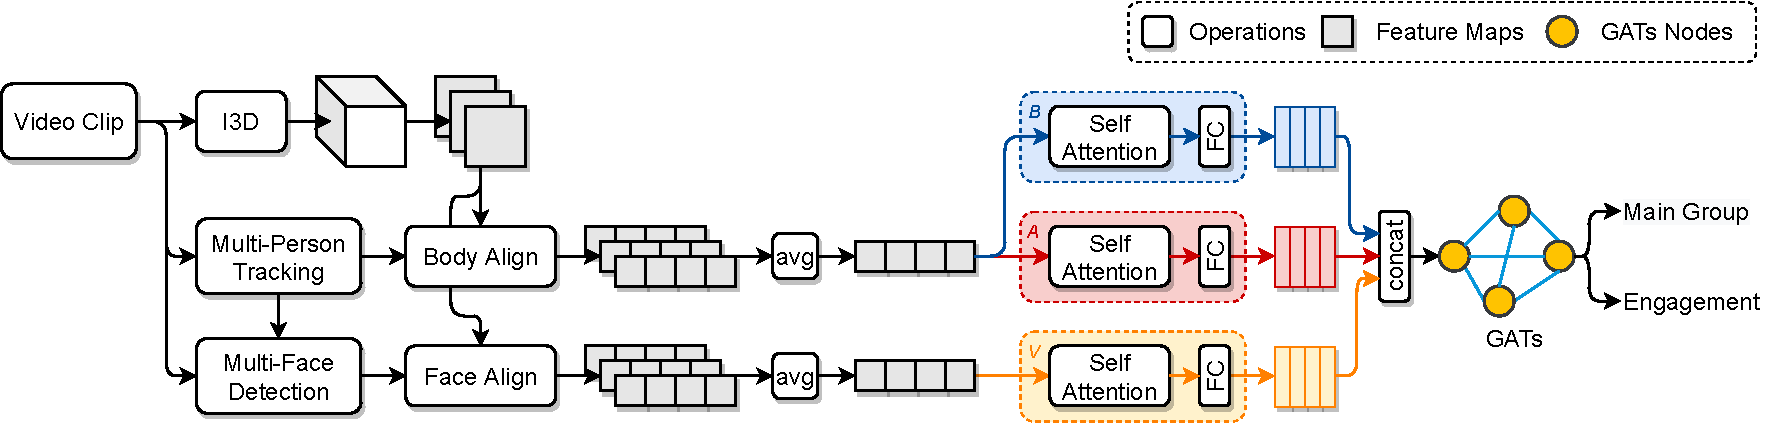
\includegraphics[width=\linewidth]{assets/pipeline_3.drawio}
  \caption{Illustration of the feature extraction and individual learning modules. We employ a I3D model for extracting individual representations. Multi-person tracking and multi-face detection are used to get the bounding boxes in order to align and slice out corresponding body and face feature maps, which are then pooled for individual learning. Three-branch self-attention mechanism is applied to refine the feature maps, \ie, learning the behavioral ($\mathcal{B}$), affective ($\mathcal{A}$), and visual ($\mathcal{V}$) engagement, respectively. The concatenation of these learned three components is the final representation of an individual.}
  \label{f:pipeline_3}
\end{figure*}

\subsection{Feature Extraction}
\label{subs:Feature_Extraction}

We use I3D as the backbone to capture the spatio-temporal context of an input video clip. In I3D, ImageNet~\cite{Deng2009ImageNet} pre-trained convolutional kernels are expanded into 3D, allowing it to seamlessly learn effective spatio-temporal representations. Motivated by the promising performance of I3D models in a wide range of video-related benchmarks, we exploit the feature representations offered by this backbone pre-trained on Kinetics 400~\cite{Kay2017Kinetics} at multiple resolutions. More specifically, we use the deep spatio-temporal feature maps ($X^G \in \mathbb{R}^{1024\times8\times7\times7}$) extracted from the final convolutional layer as a rich semantic representation describing the entire video clip. These deeper features provide low-resolution yet high-level representations that encode a summary of the video. In addition, accurate recognition of individuals' action rely on finer details which are often absent in very deep coarse representations. To extract fine spatio-temporal representations for the individuals, we use the higher resolution feature maps ($X^M \in \mathbb{R}^{832\times16\times14\times14}$) from the intermediate Mixed-4f layer of I3D. As depicted in Fig.~\ref{f:pipeline_3}, from this representation we extract three feature maps, \ie, the beginning, temporally-centered, and ending feature maps, corresponding to the beginning, center, and ending frames of the input video clip.

In addition, to eliminate the interference of redundant background information on learning, we conduct multi-person tracking and multi-face detection on the input video clips. To do that, we adopt the state-of-the-art methods ByteTrack~\cite{Zhang2021ByteTrack} and RetinaFace~\cite{Deng2020RetinaFace} to gain the bounding boxes of the bodies and faces. ByteTrack is a multi-object tracking method associating every detection box instead of only the high score ones, while the RetinaFace performs pixel-wise face localization on various scales of faces by taking advantages of joint extra-supervised and self-supervised multitask learning. Given the bounding boxes, we use RoIAlign~\cite{He2017Mask} to project the coordinates on the frames' feature maps and slice out the corresponding features for each individual's bounding box. We use an average pooling to calculate the individuals' feature maps. Formally,
\begin{equation}
  {\mathbf{F}}_m^k = AP\left(RoI\left(E\left(v_m^k\right)\right)\right)
\end{equation}
where ${\mathbf{F}}_m^k$ denoting the extracted individuals' feature maps from video clip $v_m^k$, includes participants of number $P_m^k$. $AP$, $RoI$, and $E$ are the average pooling, RoI Align, and feature extraction operations, respectively. We conduct two-level RoI align separately, \ie, $RoI = \{RoI_{body}, RoI_{face}\}$. In addition, for simplifying the notations, we will eliminate $m$ and $k$ in the following sections.

\subsection{Individual Learning}
\label{subs:Individual_Learning}

Despite being localized to the body and face bounding boxes, these representations still lack emphasis on visual clues that play a crucial role in understanding the underlying information, \eg, a person's body posture and facial expressions, which related to the behavioral, affective, and visual components of engagement. To overcome this, we adopt the self-attention mechanism~\cite{Vaswani2017Attention} to directly learn the interactions between any two feature positions of an individual's feature representation and accordingly leverage this information to refine each individual's body and face feature maps.

The self-attention module computes the response at a position in a sequence by attending to all positions and taking their weighted average in an embedding space. This mechanism was originally introduced in machine translation, but in computer vision tasks, attention mechanisms were designed to discover the important spatial regions in an image or the critical frames in a video. In our framework the self-attention module functions as a non-local operation~\cite{Wang2018NonLocal} and computes the response at each position by attending to all positions in an individual's feature map. The output of the self-attention module contextualizes the input bounding box feature map with visual clues and thus, enriches the individual's representation by highlighting the most informative features. As substantiated by ablation studies in Sec.~\ref{s:Experiments}, capturing such fine details significantly contribute to the estimation performance.

We utilize three separate self-attention modules that take the averaged body features and features as inputs. These three modules are designed to capture the behavioral ($\mathcal{B}$), affective ($\mathcal{A}$), and visual ($\mathcal{V}$) engagement. Sequentially, a fully connected (FC) layer is used to project the revised feature maps to the same size. In this step, what we expect is to learn a new representation of three engagement components from body and face maps. Finally, we concatenate each individual's features as the input of the next group learning module. The refined individual feature map is defined as
\begin{equation}
  \mathbf{H} = \left[\alpha_{\mathcal{B}}\left({\mathbf{F}_{body}}\right), \alpha_{\mathcal{A}}\left(\left[{\mathbf{F}_{body}}, {\mathbf{F}_{face}}\right]\right), \alpha_{\mathcal{V}}\left({\mathbf{F}_{face}}\right)\right].
\end{equation}

Here, $\mathbf{H} = \{h_1, ..., h_p, ..., h_P\}$ is the output from individual module and $\left[\cdot, \cdot\right]$ denotes concatenation. $\alpha$ is the attention operation.

\subsection{Group Learning}
\label{subs:Group_Learning}

Engagement estimation of the elderly relies on uncovering subtle interactions among individuals present in a multiparty HRI scenario. Based on the studies of aging faces and postures, it is not robust to estimate engagement solely from the old participant. However, it is worth noting that, in the elderly-nurse-robot interaction scenario, nurses are not only the auxiliaries and participants of the interaction, but as the people who are in daily contact with these elderly people, they have the most prompt judgment about the minor expressions of the elderly people, and these judgments will be conveyed in their behaviors. Therefore, in the HRI scenario described above, we suggest a hypothesis that \textbf{\textit{analyzing all participants in the main interaction group and the relationships between them helps us to estimate the engagement of individual elder person.}} If this hypothesis is proved true, then we can provide an answer to Q1.

Furthermore, how to identify the main interaction group in a video clip of dynamic multiparty interaction in the wild involves Q2 and Q3. According to studies for human conversation, a widely adopted classification of roles is proposed by Goffman~\cite{Goffman1981Forms}. He presented a participation structure model where each participant is assigned a participation role, \ie, speaker, addressee, and side-participant (person is part of the group of possible speakers but who currently are taking on a listening role). Clark~\cite{Clark1996Using} further made a distinction between participants and non-participants. The former includes speaker, addressee, and side-participant, while the latter includes bystanders and overhearers. By using this concept to classify the detected people into main group and background, we are able to solve Q2 and Q3 if we find an automated approach.

In order to solve the above questions, we propose a group learning module. This problem can elegantly be modeled by a graph. Graph neural networks (GNNs)~\cite{Scarselli2008Graph} allow graph representations to be learned with neural networks, which were originally developed for structured data, but have recently been generalized to various computer vision tasks. In a graph, the nodes represent refined individuals' feature maps and the edges represent the interactions among individuals. Typically, graph-based models employ the information from neighbor points according to the characteristics of the specific task, \ie, compute the hidden representations of each node in the graph, by attending over its neighbors. We adopt the recently proposed GATs~\cite{Velivckovic2017Graph} to directly learn the underlying interactions and seamlessly capture the global activity context. GATs flexibly allow learning attention weights between nodes through parameterized operations based on a self-attention strategy and have successfully demonstrated state-of-the-art results by outperforming existing counterparts. 

We construct our graph attention layer (GAL) as following. The input of our GAL is $\mathbf{H} = \{h_1, ..., h_p, ..., h_P\}$, where $P$ is the number of nodes. The layer produces a new set of node features $\mathbf{H}^{\prime}  = \{h_1^{\prime}, ..., h_p^{\prime}, ..., h_P^{\prime}\}$ as its output. Initially, a shared linear transformation with the weight matrix $W$ is applied to every node. We then perform a shared self-attention mechanism $a$ to compute attention coefficients
\begin{equation}
  e_{ij} = a\left(Wh_i,Wh_j\right)
\end{equation}
that indicate the importance of node $j$'s features to node $i$. The model allows every node to attend on other nodes. To make coefficients easily comparable across different nodes, we normalize them across all choices of $j$ using the softmax function:
\begin{equation}
  \alpha_{ij} = {\rm softmax}_j(e_{ij}) = \frac{{\rm exp}(e_{ij})}{\sum_{k \in \mathcal{N}}{\rm exp}(e_{ik})}.
\end{equation}

In our experiments, the attention mechanism $a$ is a single-layer feedforward neural network, parameterized by a weight vector $\mathbf{a}$, and applying the LeakyReLU nonlinearity (with negative input slope $\alpha = 0.2$). Fully expanded out, the coefficients computed by the attention mechanism (illustrated by Fig.~\ref{f:gats}) may then be expressed as:
\begin{equation}
  \alpha_{ij} = \frac{{\rm exp}({\rm LeakyReLU}(\mathbf{a}^T[Wh_i,Wh_j]))}{\sum_{k \in \mathcal{N}}{\rm exp}({\rm LeakyReLU}(\mathbf{a}^T[Wh_i,Wh_k]))}.
\end{equation}

\begin{figure}[t]
  \centering
  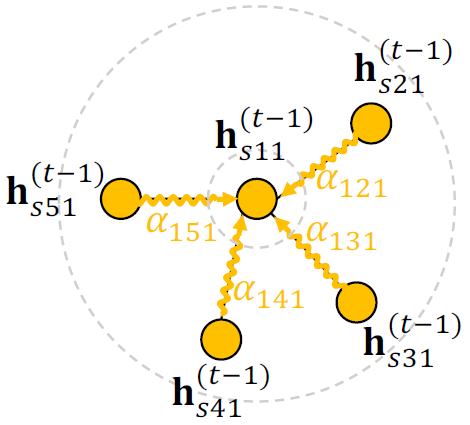
\includegraphics[width=0.4\linewidth]{assets/gats}
  \caption{An illustration of Graph Attention Networks by node 1 on its neighborhood. Different arrow styles and colors denote independent attention computations. The aggregated features from each head are concatenated or averaged to obtain $h_1^{\prime}$.}
  \label{f:gats}
\end{figure}

Once obtained, the normalized attention coefficients are used to compute a linear combination of the features corresponding to them, to serve as the final output features for every node (after potentially applying a nonlinearity, $\sigma$):
\begin{equation}
  h_i^{\prime} = \sigma\left(\sum_{j \in \mathcal{N}} \alpha_{ij}Wh_j\right).
\end{equation}

To stabilize the learning process of self-attention, we have found extending our mechanism to employ multi-head attention to be beneficial. Specifically, K independent attention mechanisms execute the transformation of Equation 4, and then their features are concatenated, resulting in the following output feature representation:
\begin{equation}
  h_i^{\prime} = \left[\sigma\left(\sum_{j \in \mathcal{N}} \alpha_{ij}^kW^kh_j\right)\right]_{k=1 \to K}.
\end{equation}
$\alpha_{ij}^k$ is normalized attention coefficients computed by the $k$-th attention mechanism ($a^k$), and $W^k$ is the corresponding input linear transformation's weight matrix.

Specially, if we perform multi-head attention on the final (prediction) layer of the network, concatenation is no longer sensible—instead, we employ averaging, and delay applying the final nonlinearity (usually a softmax or logistic sigmoid for classification problems) until then
\begin{equation}
  h_i^{\prime} = \sigma\left(\frac{1}{K}\sum_{k=1}^K\sum_{j \in \mathcal{N}} \alpha_{ij}^kW^kh_j\right).
\end{equation}

The aggregation process of a multi-head graph attentional layer is illustrated by Fig.~\ref{f:gats}.

GATs compute attention coefficients for every possible pair of nodes, which can be represented in an adjacency matrix $\hat{O}^\alpha$.

\subsection{Engagement Estimator}
\label{subs:Engagement_Estimator}

After the model is trained, we can perform two types of group-based re-id tasks. Specifically, the graph-level representations from the readout attention module are directly employed for group re-id. For group-aware person re-id, the node-level features already contain discriminative context information as they receive messages from both intra-group and inter-group members. In addition, we can also utilize the person correspondence learning module to further reduce the ambiguity between people with similar appearances. The inference of group re-id and group-aware person re-id can be jointly computed in our framework. The results of group re-id and group-aware person re-id are discussed in Sec.~\ref{s:Experiments}, respectively.

In our framework, the GAT module consumes the individuals' feature maps obtained from the self-attention component, encodes inter-node relations, and generates an updated representation for each individual. We acquire the group representation by max-pooling the enriched individuals' feature map and adding back a linear projection of the holistic video's features obtained from the I3D backbone. A classifier is then applied on this representation to generate group activity scores denoted by $\hat{O}^G$. Similarly, another classifier is applied on the individuals' representation to govern the individual action scores denoted by $\hat{O}^I_n$. The associated operations provide a fully differentiable mapping from the input video clip to the output predictions, allowing the framework to be trained in an end-to-end fashion by minimizing the following objective function,
\begin{equation}
\mathcal{L} = \mathcal{L}_{gp}(O_G,\hat{O}^G)+\lambda \sum_{} \mathcal{L}_{ind} (O^I_n,\hat{O}^I_n)
\end{equation}
where $\mathcal{L}_{gp}$ and $\mathcal{L}_{ind}$ respectively denote the cross-entropy loss for group activity and individual action classification. Here, $\hat{O}^G$ and $\hat{O}^I$ n represent the ground-truth group activities and individual actions, $n$ identifies the individual and $\lambda$ is the balancing coefficient for the loss functions.

% ========================= DATASETS ============================
\section{Datasets}
\label{s:Datasets}

It is still challenging for researchers to adequately investigate and explore the interaction between old people and a robot. The barriers can be divided into three parts. First, in order to understand how older people interact with robots, researchers must have a robot with basic build-in vision and language capabilities. Many small research groups cannot afford the cost. Second, researchers need to find sufficient samples (elderly people) participating in the experiments. Data collection is also very difficult due to safety and privacy concerns. Third, there is no publicly available dataset or benchmark in our research community, which makes the comparison and discussion difficult to achieve.

We have 21 interaction sessions in a span of 4 months with over 15 older people attending the experiments. The IMI-BHEH dataset has the following contributions
\begin{itemize}
  \item IMI-BHEH dataset is collected in the free old-people-robot interaction scenario. There is no constraint imposed on the participants. The elderly talk to a humanoid robot while the nurses occasionally provide help.
  \item The participants of IMI-BHEH dataset are people with dementia. To the best of our knowledge, there is no publicly available dataset aiming to study their behaviors and interaction with robots.
  \item IMI-BHEH dataset is collected in a wild, dynamic, and multiparty environment. In the background, nurses may pass through the scene; some old people may sit near to or far from the interaction group; the interaction participants may leave and join at any time. All of these make the data more realistic.
\end{itemize}

Our dataset includes annotations as described in Table.~\ref{t:dataset}. 2D people bounding box is automatically annotated by Yolo5\footnote{https://github.com/ultralytics/yolov5}. 2D skeleton information and reconstructed 3D skeleton information are extracted using [5]. Facial landmarks and AUs are extracted from [6]. It is noteworthy that previously mentioned features are manually checked. The main interaction group participant ID and bounding box are annotated by professional volunteers. The label of the data is the engagement score, which is gained from a revised version of the engagement psychometric scale of people with dementia [7]. The details can be found in Appendix~\ref{ap:annotation_form}.


\begin{table}[t]
  \renewcommand{\arraystretch}{1.3}
  \centering
  \caption{Details of IMI-BHEH Dataset}
  \label{t:dataset}
  \begin{tabular}{ccc}
  \toprule
  \textbf{Raw Data} &
  \textbf{Extracted Features} &
  \textbf{Label}\\
  \midrule
  \multirow{6}{*}{Videos} & 2D people bounding box & \multirow{6}{*}{Engagement} \\
  & 2D skeleton & \\
  & Reconstructed 3D skeleton & \\
  & Facial landmarks and AUs & \\
  & Main group participant ID & \\
  & Main group 2D bounding box & \\
  \bottomrule
  \end{tabular}
\end{table}

% ======================== EXPERIMENTS ==========================
% 1. Implementation Details
% 2. Results and Discussions
\section{Experiments}
\label{s:Experiments}

\subsection{Implementation Details}
\label{subs:Implementation_Details}

In our model, we use an I3D backbone which is initialized with Kintetics-400 [32] pre-trained model. We utilize ROI-Align with crop size of $5\times5$ on extracted feature-map from Mixed-4f layer of I3D. We perform self-attention on each individuals' feature map with query, key and value being different linear projections of individuals' feature map with output sizes being $1/8$, $1/8$, $1$ of the input size. We then learn a 1024-dim feature map for each individual features obtained from self-attention module. Aligned individuals' feature maps are fed into our single-layer, multi-head GAT module with 8 heads and input-dim, hidden-dim, output-dim being 1024 and dropout probability of 0.5 and $\alpha = 0.2$ [60]. We utilize ADAM optimizer with $\beta_1 = 0.9$, $\beta_2 = 0.999$, $\epsilon = 10^{-8}$ following [65]. We train the network in two stages. First, we train the network without the graph attention module. Then we fine-tune the network end-to-end including GAT. For the Volleyball dataset, we train the network in 200 epochs with a mini-batch size of 3 and a learning rate ranging from $10^{-4}$ to $10^{-6}$ and $\lambda_1 = 8$. For the CAD, we train the network in 150 epochs with a mini-batch size of 4 and a learning rate ranging from $10^{-5}$ to $10^{-6}$ and $\lambda_1 = 10$. Input video clips to the model are 17 frames long, with the annotated key frame in the center. At test time, we perform our experiments based on two widely used settings in group activity recognition literature namely ground truth-based and Detection-based settings. In the ground truth-based setting, ground-truth bounding boxes of individuals are given to the model to infer the individual action for each box and the group activity for the whole scene. In the detection based setting, we fine-tune a Faster-RCNN [46] on both datasets and utilize the predicted boxes for inferring the individuals' action and group activity.

% \subsection{Evaluation Metrics}
% \label{subs:Evaluation_Metrics}

% \subsection{Ablation Studies}
% \label{subs:ablation_studies}

% \subsection{Results and Discussion}
% \label{subs:Results_and_Discussion}


% ======================== CONCLUSIONS ==========================
% 1. Summary the proposed approach
% 2. Results
% 3. Limitations and Future Work
\section{Conclusions}
\label{s:Conclusions}

\textcolor{red}{Human behavior and social signal understanding have achieved good performance in the computer vision area. However, most of them are based on the analysis of an individual subject and are achieved in experimental settings. In this paper, we use real-world and open-world image data to estimate the engagement of old people in a multiparty human-robot interaction scenario. For this purpose, we place a humanoid robot in a non-profit nursing home, where the elderly are accompanied by nurses and engage in spontaneous conversations with the robot. We perform the analysis and feature extraction on three scales, namely global, group, and individual, which gradually reduce via people detection, main group detection, and the old people localization. We propose a multi-branch network with attention and graphic convolutional layers combining three-level information. Our experiments show that the proposed framework achieves good performance in the engagement estimation task.}

% ======================== APPENDICES ===========================
% Single appendix:
% \appendix[Appendix Title]  % has heading
% \appendix                  % no heading
% Two or more appendices:
% \appendices
% \section{Appendix Title}   % Appendix one text goes here.
% \section{}                 % Appendix two text goes here.
\appendix
\label{ap:annotation_form}

We used a revised version of EPWDS for artificial engagement annotation. The form for annotators are appended in Fig.~\ref{f:annotation_form}.

\begin{figure*}[ht]
  \centering
  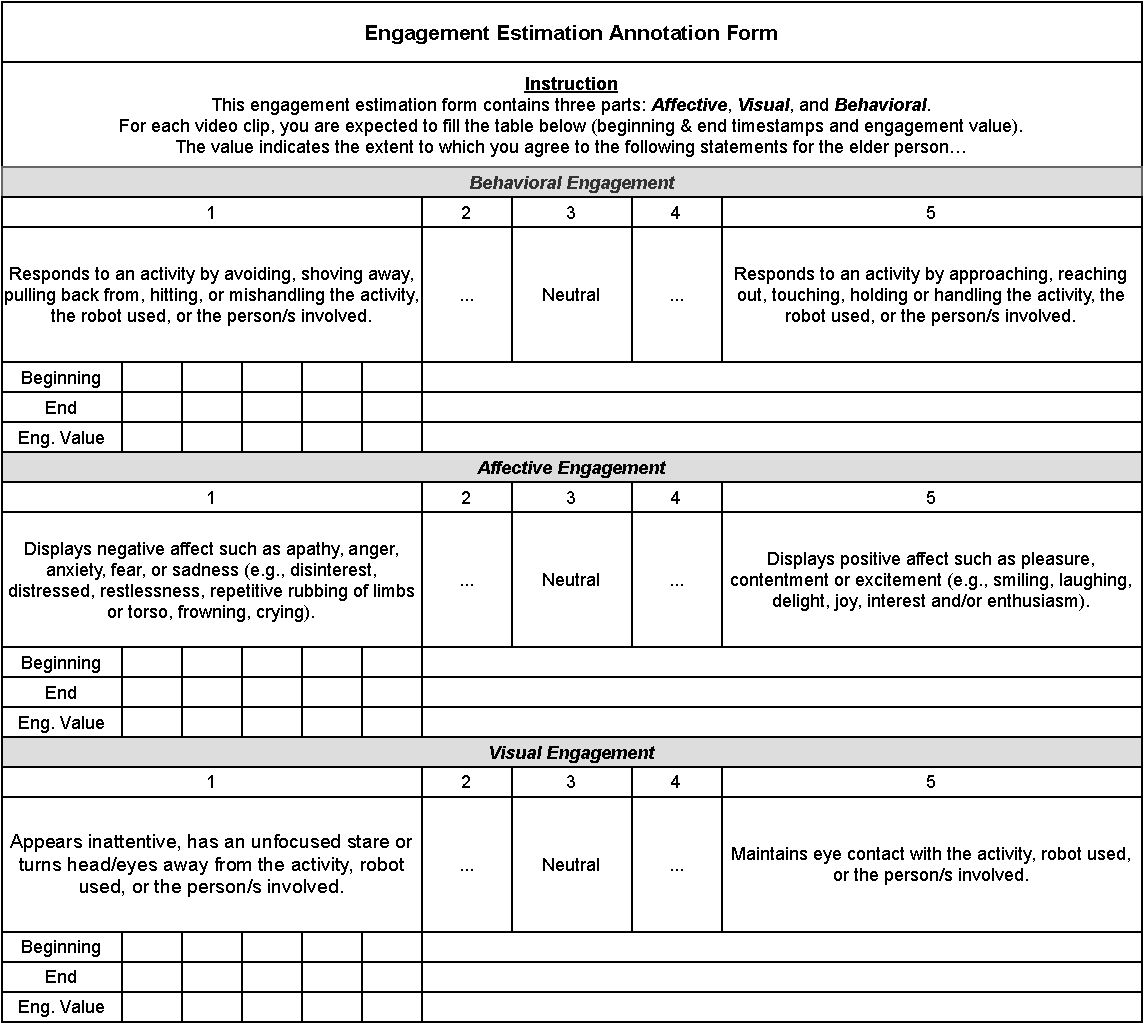
\includegraphics[width=\linewidth]{assets/annotation_form.drawio}
  \caption{Engagement Estimation Annotation Form}
  \label{f:annotation_form}
\end{figure*}

% ====================== ACKNOWLEDGMENTS ========================
% \section*{Acknowledgments}


% ======================== REFERENCES ===========================
% Put references on a page by themselves when using endfloat and
% the captionsoff option:
\ifCLASSOPTIONcaptionsoff
  \newpage
\fi
% \IEEEtriggeratref{8}
% The "triggered" command can be changed if desired:
% \IEEEtriggercmd{\enlargethispage{-5in}}

\bibliographystyle{IEEEtran}
\bibliography{IEEEabrv,TAC}


% ========================= BIOGRAPHY ===========================
% If you have an EPS/PDF photo extra braces are needed around
% the contents of the optional argument to biography to prevent
% the LaTeX parser from getting confused when it sees the
% complicated \includegraphics command within an optional
% argument. (You could create your own custom macro containing
% the \includegraphics command to make things simpler here.)
% Or if you just want to reserve a space for a photo:

% \begin{IEEEbiography}[{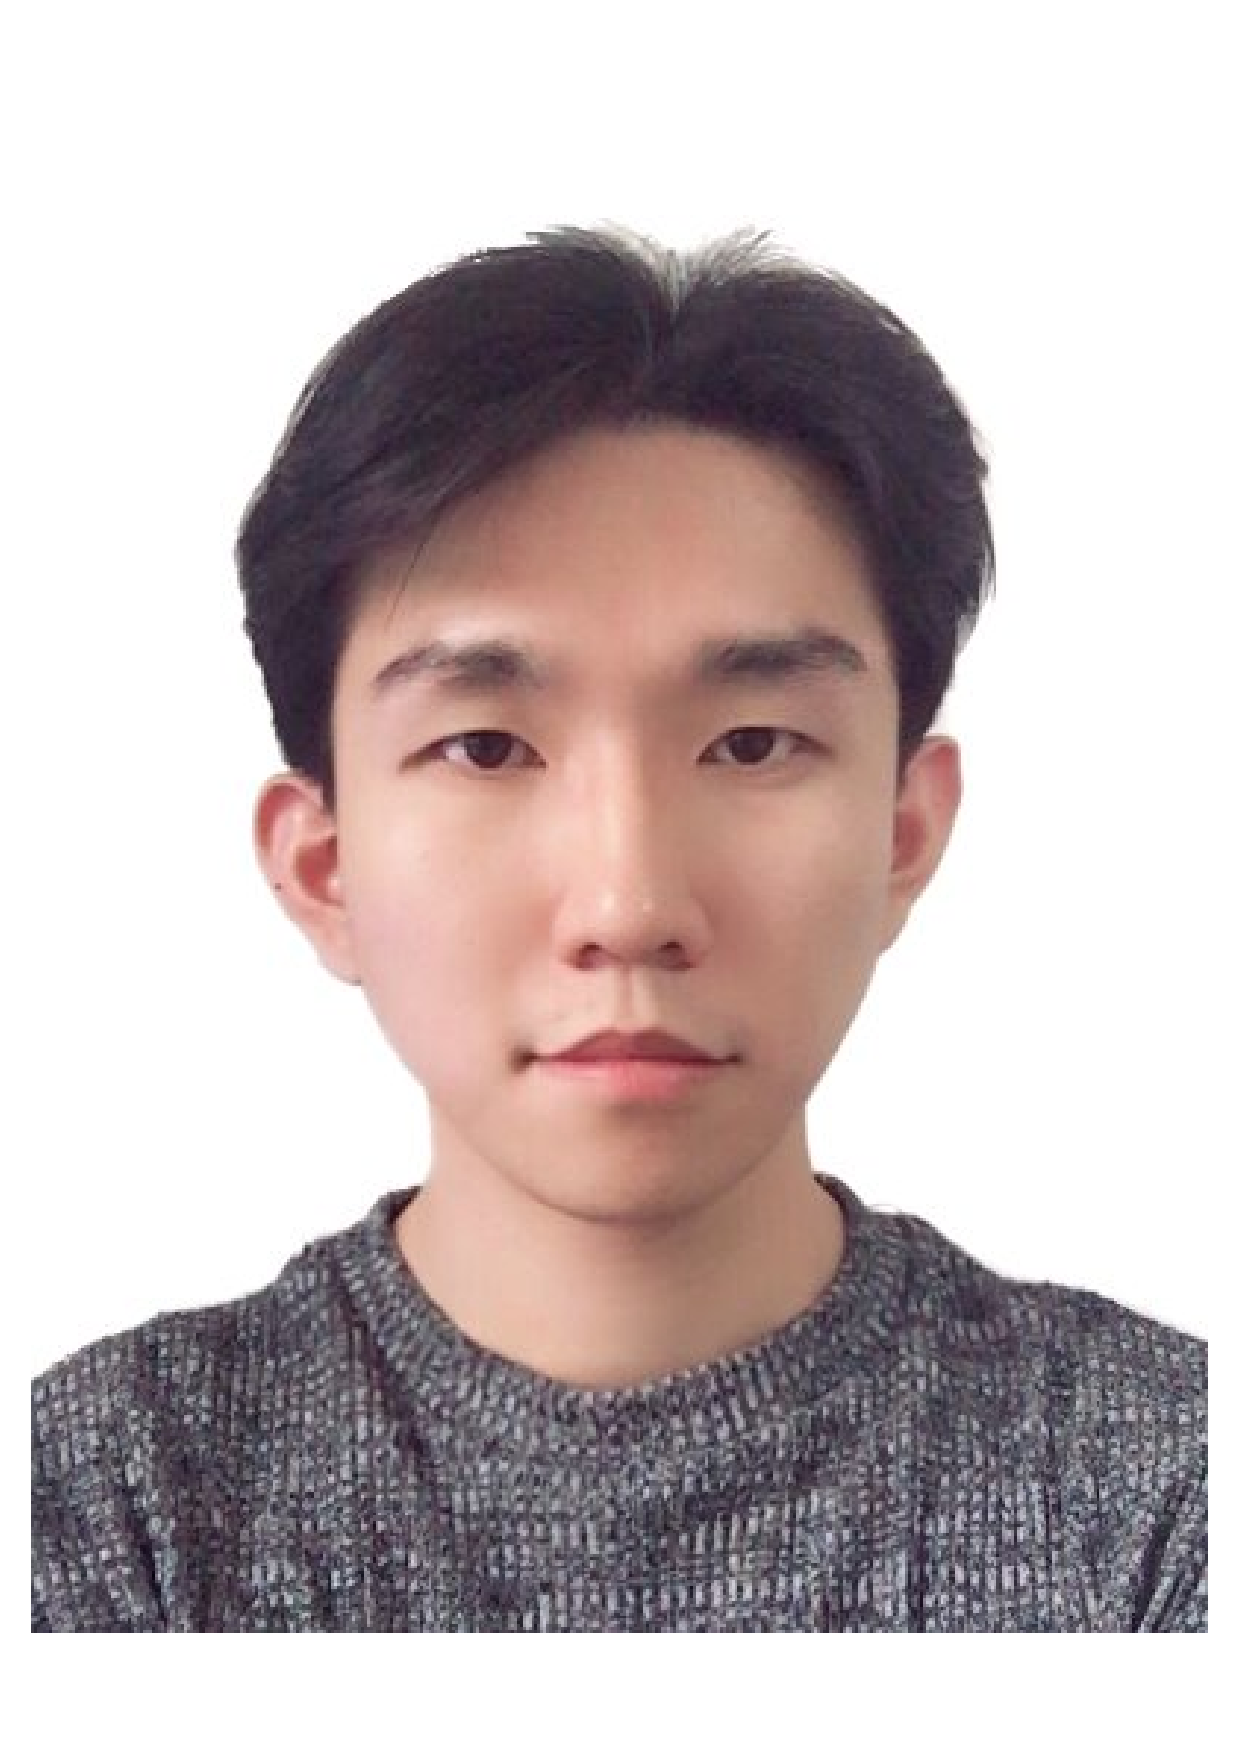
\includegraphics[width=1in,height=1.25in,clip,keepaspectratio]{zhijie_zhang}}]{Zhijie Zhang}
\begin{IEEEbiography}{Zhijie Zhang}
  Biography text here.
\end{IEEEbiography}

\begin{IEEEbiography}{Jianmin Zheng}
  is a professor in the School of Computer Science and Engineering at Nanyang Technological University, Singapore. He received the BS and Ph.D. degrees from Zhejiang University, China. His recent research focuses on T-spline technologies, digital geometric processing, reality computing, AR/VR, and AI assisted part design for 3D printing. He is currently the program director for the research pillar of ML/AI under the HP-NTU Digital Manufacturing Corporate Lab. He is also a member of executive committee of AsiaGraphics Association.
\end{IEEEbiography}

\begin{IEEEbiography}{Nadia Magnenat Thalmann}
  (Member, IEEE) received her bachelor's and master's degrees in psychology, biology, chemistry, and computer science, and the Ph.D. degree in quantum physics from the University of Geneva. She is currently the Director of the Virtual Humans and Social Robotics Research Laboratory, MIRALab, University of Geneva. From 2009 to 2021, she was the Director of the Institute for Media Innovation, NTU, Singapore. In NTU, she revolutionized social robotics by unveiling the first social robot Nadine that can have mood and emotions and remember people and actions. She is a Life Member of the Swiss Academy of Engineering Sciences. She received honorary doctorates from Leibniz University of Hannover and the University of Ottawa, Canada, and several prestigious other awards as the Humboldt Research Award in Germany. She is the Editor-in-Chief of The Visual Computer and the Co-Editor-in-Chief of Computer Animation and Virtual Worlds.
\end{IEEEbiography}

% insert \newpage where needed to balance the two columns on the
% last page with biographies:
% \newpage

% You can push biographies down or up by placing a \vfill before
% or after them. The appropriate use of \vfill depends on what
% kind of text is on the last page and whether or not the
% columns are being equalized.
% \vfill

% Can be used to pull up biographies so that the bottom of the
% last one is flush with the other column.
% \enlargethispage{-5in}

\end{document}
